%!TEX root = ../my_thesis.tex

\chapter{Les codes polaires}

Résumé

\vspace*{\fill}
\minitocTITI
\vspace*{\fill}

\subsection*{Introduction}

\section{Principe et construction}

\subsection{Contexte}



\begin{figure}[t]
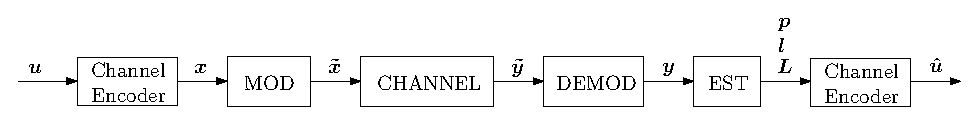
\includegraphics{main/ch1_fig/chaine_com2}
\caption{Une chaîne de communication}
\label{fig:chaine_com}
\end{figure}
Une chaîne de communications numériques est représentée en Figure \ref{fig:chaine_com}.
Elle représente les étapes usuelles de la transmission de données numériques depuis une \textbf{source} vers un \textbf{destinataire} à travers un \textbf{canal}.
Le canal de transmission est le support qui permet le transfert de l'information. Ce canal peut être une paire de cable au sein duquel un signal électrique transporte l'information. Le milieu aquatique traversé par des ondes accoustiques portant de l'information en est également un. Même le vide, par lequel passent les ondes émises par les antennes de nos satellites, peut constituer un canal de transmission.
Dans les trois exemples précédents, les grandeurs physiques associées aux supports de l'information sont continues tandis que les données à transmettre, dans le cadre des communications numériques, sont discrètes. Le rôle du modulateur est de transformer l'information discrète en signaux physiques transmissibles par le canal. Dans le cas de signaux électriques, il s'agira de formes d'ondes. 

% Problèmes : 
% - introduire d'ores et déjà les notions d'alphabet
% - postuler des binaires pour simplifier le discours ?
% - parler d'encodage source ?
% - Intérêt du canal sous-marin à part faire bling bling ?
% - Info souple / dure ?
% - Définition Taux d'erreur binaire / taux d'erreurs trame
% - Gras sur séquence d'information et mot de code
% - Définir le rendement

Dans le canal de communication, ces signaux subissent de nombreuses perturbations. Les composants circuits électriques qui réalisent la fonction de modulation, les interférences causées par d'autres utilisateurs du canal en sont des exemples. Aussi, le démodulateur, qui analyse les signaux reçus en sortie du canal, ne peut donner que des estimations des symboles envoyés par le modulateur. En l'absence de traitement supplémentaire, dans le cas d'un canal fortement bruité, la chaine de communications décrite ici présenterait un taux d'erreur binaire (TEB) élevé : les bits en sorties de la chaîne seraient fréquemment différents des bits de la séquence d'information.

L'ajout d'un encodeur et d'un décodeur canal dans la chaîne de transmission est moyen efficace de réduire ce taux d'erreur. L'encodeur transforme une séquence d'information de $K$ bits en un \textbf{mot de code} de $N$ bits présentant de la redondance. Le décodeur canal, ou parfois le couple démodulateur - décodeur canal, utilise cette redondance pour améliorer le taux d'erreur binaire de la chaîne de transmission. Dans la présente thèse, le décodeur canal est découplé du démodulateur. L'ensemble modulateur - canal - démodulateur peut être considéré comme une entité indépendante dont l'entrée est le mot de code et la sortie une séquence d'estimation. Cet ensemble est appelé canal composite.
% Ici je parle de flux binaire alors qu'avant d'ensemble discret en général

\subsection{Le modèle mathématique}
La modulation considérée est une modulation à changement de phase binaire (BPSK) qui associe aux valeurs binaires d'entrée $x\in\{0,1\}$ les valeurs réelles $\hat{x}\in\{-1,1\}$, respectivement.
Le canal à bruit blanc additif gaussien à double entrée (BI-AWGNC) tel que défini dans \cite[Section~1.5.1.3]{ryan2009channel} est le seul considéré. Ce modèle est le plus utilisé pour caractériser les performances des codes correcteurs d'erreur car il se rapproche du bruit thermique évoqué précédemment, qui est souvent prépondérant. La puissance du bruit est quantifiée par $N_0$, la densité spectrale mono-latérale du bruit blanc gaussien. Afin d'évaluer les performances de correction des codes correceurs d'erreurs, les taux d'erreur seront souvent rapportés au \textbf{rapport signal à bruit} (SNR), noté $E_b/N_0$, où $E_b=\mathbb{E}(\hat{x}^2)$ est l'énergie moyenne par bit d'information.

Les estimations en sortie du décodeur sont données sous la forme de rapport de vraisemblance logarithmique. Leur signe détermine la valeur binaire d'entrée $x$ la plus probable, et leur valeur absolue le degré de fiabilité de cette valeur d'entrée.





% Ajouter des maths ;D


\begin{itemize}
\item Chaine de communication : complet -> simplifié data -> encodeur -> canal -> décodeur-data
\item Introduire redondance
\item Codes linéaires - codes en blocs : évocation de certains pour exemple (hamming ? ldpc ?)
\item Info souple / dure

\end{itemize}
\subsection{Noeuds de parité et d'égalité}
\begin{itemize}
\item Codes bloc : réseau parité et égalité (reprendre exemple)
\item Dans codes polaires, noyau 2 utilisé
\item donner les équations
\end{itemize}
\subsection{Polarisation}
\begin{itemize}
\item donner comportement pour bec
\item recursivité -> matrice ou factor graph d'un code polaire complet
\item simulations, représentation de la polarisation
\end{itemize}
\subsection{Constructions des codes polaires}
\begin{itemize}
\item puisque polarisation -> bits gelés
\item equations SC
\end{itemize}

\section{Les algorithmes de décodage de codes polaires}

\subsection{Annulation Successive}
\begin{itemize}
\item Séquencement
\item Parallélisme
\end{itemize}
\subsection{Annulation Successive Liste}
\begin{itemize}
\item Algorithme
\item Calcul Métrique

\end{itemize}
\subsection{Algorithmes itératifs à sortie souple}
\begin{itemize}
\item Noeud 2 à sortie souple
\item BP
\item SCAN
\end{itemize}

\subsection{Autres algorithmes}
\begin{itemize}
	\item SCS
	\item SCF
\end{itemize}
\section{Améliorations algorithmiques}

\subsection{Elagage de l'arbre de décodage}

\subsubsection{Fast SC}
\begin{itemize}
\item R0 - R1
\item SPC - REP
\item détailler calculs évitables (g0, f0, grep)
\end{itemize}
\subsubsection{Fast SCL}
\begin{itemize}
\item détailler adaptation élagage pour SC Liste - calculs métriques
\item discussion chase spc - r1 ? Hashemi-Sarkis + Simulations
\end{itemize}
\subsubsection{Fast SCAN}
\begin{itemize}
\item 
\end{itemize}

\subsection{Adaptive}

\section{Codes polaires de taille variables}
% https://arxiv.org/pdf/1701.06458.pdf 4-5-6-7-8-9


\subsection*{Conclusion}
